\section{Methodology Description}
\label{S:T4}
Pedestrian's movement patterns are highly correlated both temporally and spatially ~\citep{song2016deeptransport}. Treating mobility patterns of pedestrians as a sequence prediction problem, Recurrent Neural Networks (RNN) is a popular choice to deal with the problem.  However, it's been shown that RNN's are not capable of remembering long-term temporal and spatial dependencies as a result of the problem of vanishing gradient. \citep{hochreiter1997long}. Introduced in \citep{hochreiter1997long}, Long Short-Term Memory (LSTM), is a modification to traditional RNN architecture that enables learning sequence labels for longer time intervals by implementing four interactive gates. In Figure \ref{fig:LSTM}, a schematic framework of an LSTM is depicted. To compute a sequence of output units \(Y=(y_1,y_2,...,y_T)\), from a sequence of input \(X=(X_1,X_2,...X_T)\), the following equations should be followed iteratively over time \textit{t}:
\begin{enumerate}
    \item forget gate: \(f_t=\sigma(W_fx_t+U_fh_{t-1}+b_f)\)
    \item input gate: \(i_t=\sigma(W_ix_t+U_ih_{t-1}+b_i)\)
    \item Cell state: \(c_t=f_t\odot c_{t-1}+i_t\odot \sigma(W_cx_t+U_ch_{t-1}+b_c) \)
    \item output gate: \(o_t=\sigma(W_ox_t+U_oh_{t-1}+b_o)\)
    \item hidden state: \(h_t=o_t\odot \sigma(c_t)\)
    \item output layer: \(y_t=\sigma(W_{y}h_t+b_y)\)
\end{enumerate}
in which: \(f_t,i_t,o_t\) are the activation vectors of forget gate, input gate and output gate respectively. \(h_t\) is the hidden state vector, which plays the role of an output vector of LSTM unit, \(c_t\) is the cell state vector, \(W,U\) and \(b\) are the weights and biases to be learned in the training phase, and \(\odot\) represents the element-wise product. \(\sigma\) represents the activation functions on respective layers. 
\begin{figure}[!h]
    \centering
    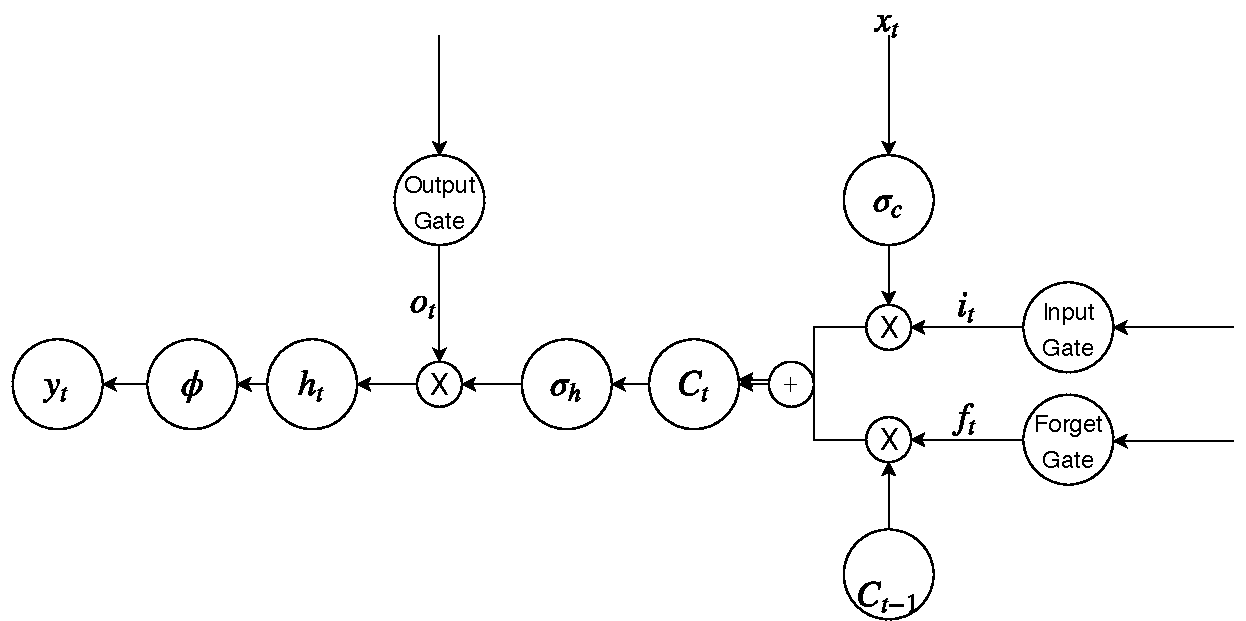
\includegraphics[scale=0.6]{chapter_6/figures/lstm.pdf}
    \caption{Schematic framework of an LSTM block}
    \label{fig:LSTM}
\end{figure}

In this study, we are proposing, \textit{Aux-LSTM}, a novel framework consisting of multi-input LSTM layers and fully connected dense layers, to predict multi-step outputs. Initial steps of time-series data, i.e. coordinates, head orientations, and distance to vehicle, are used as input to LSTM layers. The output of the LSTM layers will then merge with extra information from environmental variables, and enters to a series of fully connected dense layers to predict the multi-step trajectory of the pedestrians in the rest of their crossing. The proportion of data that is used as input, \(p\), can be adjusted and is defined as the proportion of lane width that the pedestrian has passed when the vehicle tries to predict the rest of the trajectory. For instance, if \(p\) is set to 0.3, the framework tries to predict the trajectory of the pedestrians based on their trajectory in the first 30\% of the lane width. As a regularization mechanism to the framework, the model is supervised through two identical loss functions. Both loss functions are defined as the euclidean distance between predicted and actual coordinates. By using the loss function after the LSTM layers, a.k.a. secondary loss, we allow a smoother training for the framework. Batch Normalization and Dropout layers are also used in order to reduce overfitting in the model. Figure~\ref{fig:frame} depicts the general framework of Aux-LSTM.
\begin{figure}[!h]
    \centering
    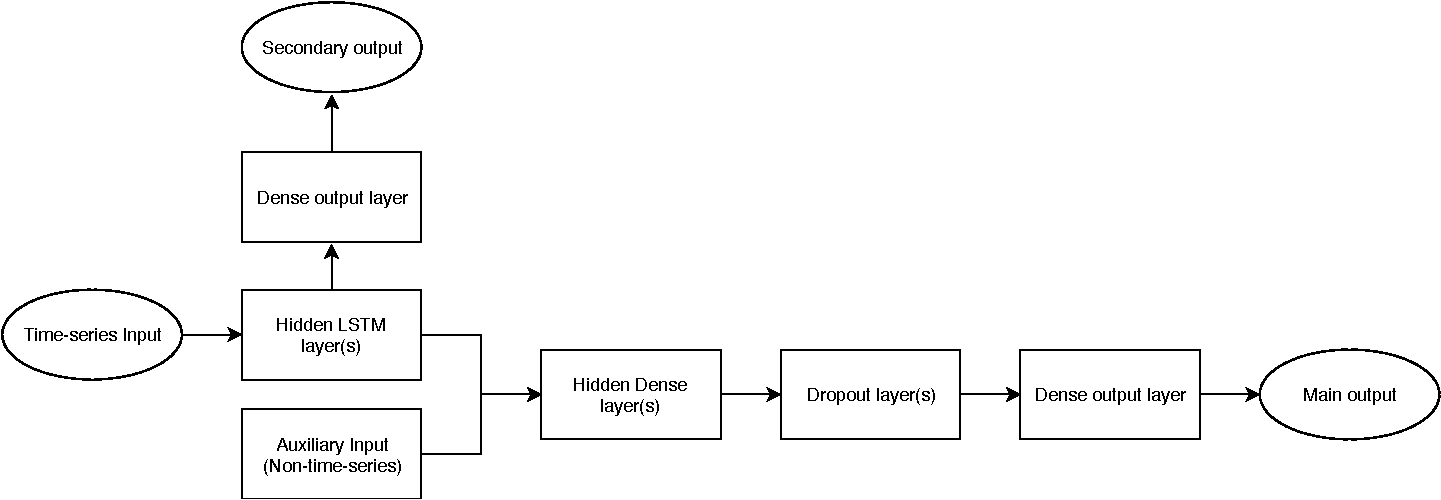
\includegraphics[scale=0.6]{chapter_6/figures/frame.pdf}
    \caption{Schematic framework of Aux-LSTM}
    \label{fig:frame}
\end{figure}